\section{Work Environment Example}
The following is a typical use case for the system whose implementation has been described in Section \ref{ch:System Implementation}.

To begin with, a regular house configuration is taken into account, as shown in Figure \ref{blueprint_deployment}. The ESP nodes are placed in the living room, in the bedroom and in the backyard, by way of example. The Raspberry Pi is located near the wireless router: this opens the possibility of using a wired connection to interface to the router itself.

All the boards must be able to connect to the AP and must be in its coverage range to work properly. Their electrical configuration and purpose is the following:

\begin{itemize}
	\item \textbf{Raspberry Pi:} connected to the AC mains and placed near the wireless router. It must be always up and running to provide the user interface and the MQTT broker functionality;
	\item \textbf{Backyard ESP-12E:} hooked up to a battery and uses deep sleep to reduce the power consumption;
	\item \textbf{Living Room ESP-32:} wired to the AC mains and always active because it is in charge of controlling the living room lamp near the couch;
	\item \textbf{Bedroom ESP-12E:} its power source can be either a battery or the AC mains depending on the availability of power outlets nearby. It uses deep sleep to save energy.
\end{itemize}


\begin{figure}[H]
	\begin{center}
		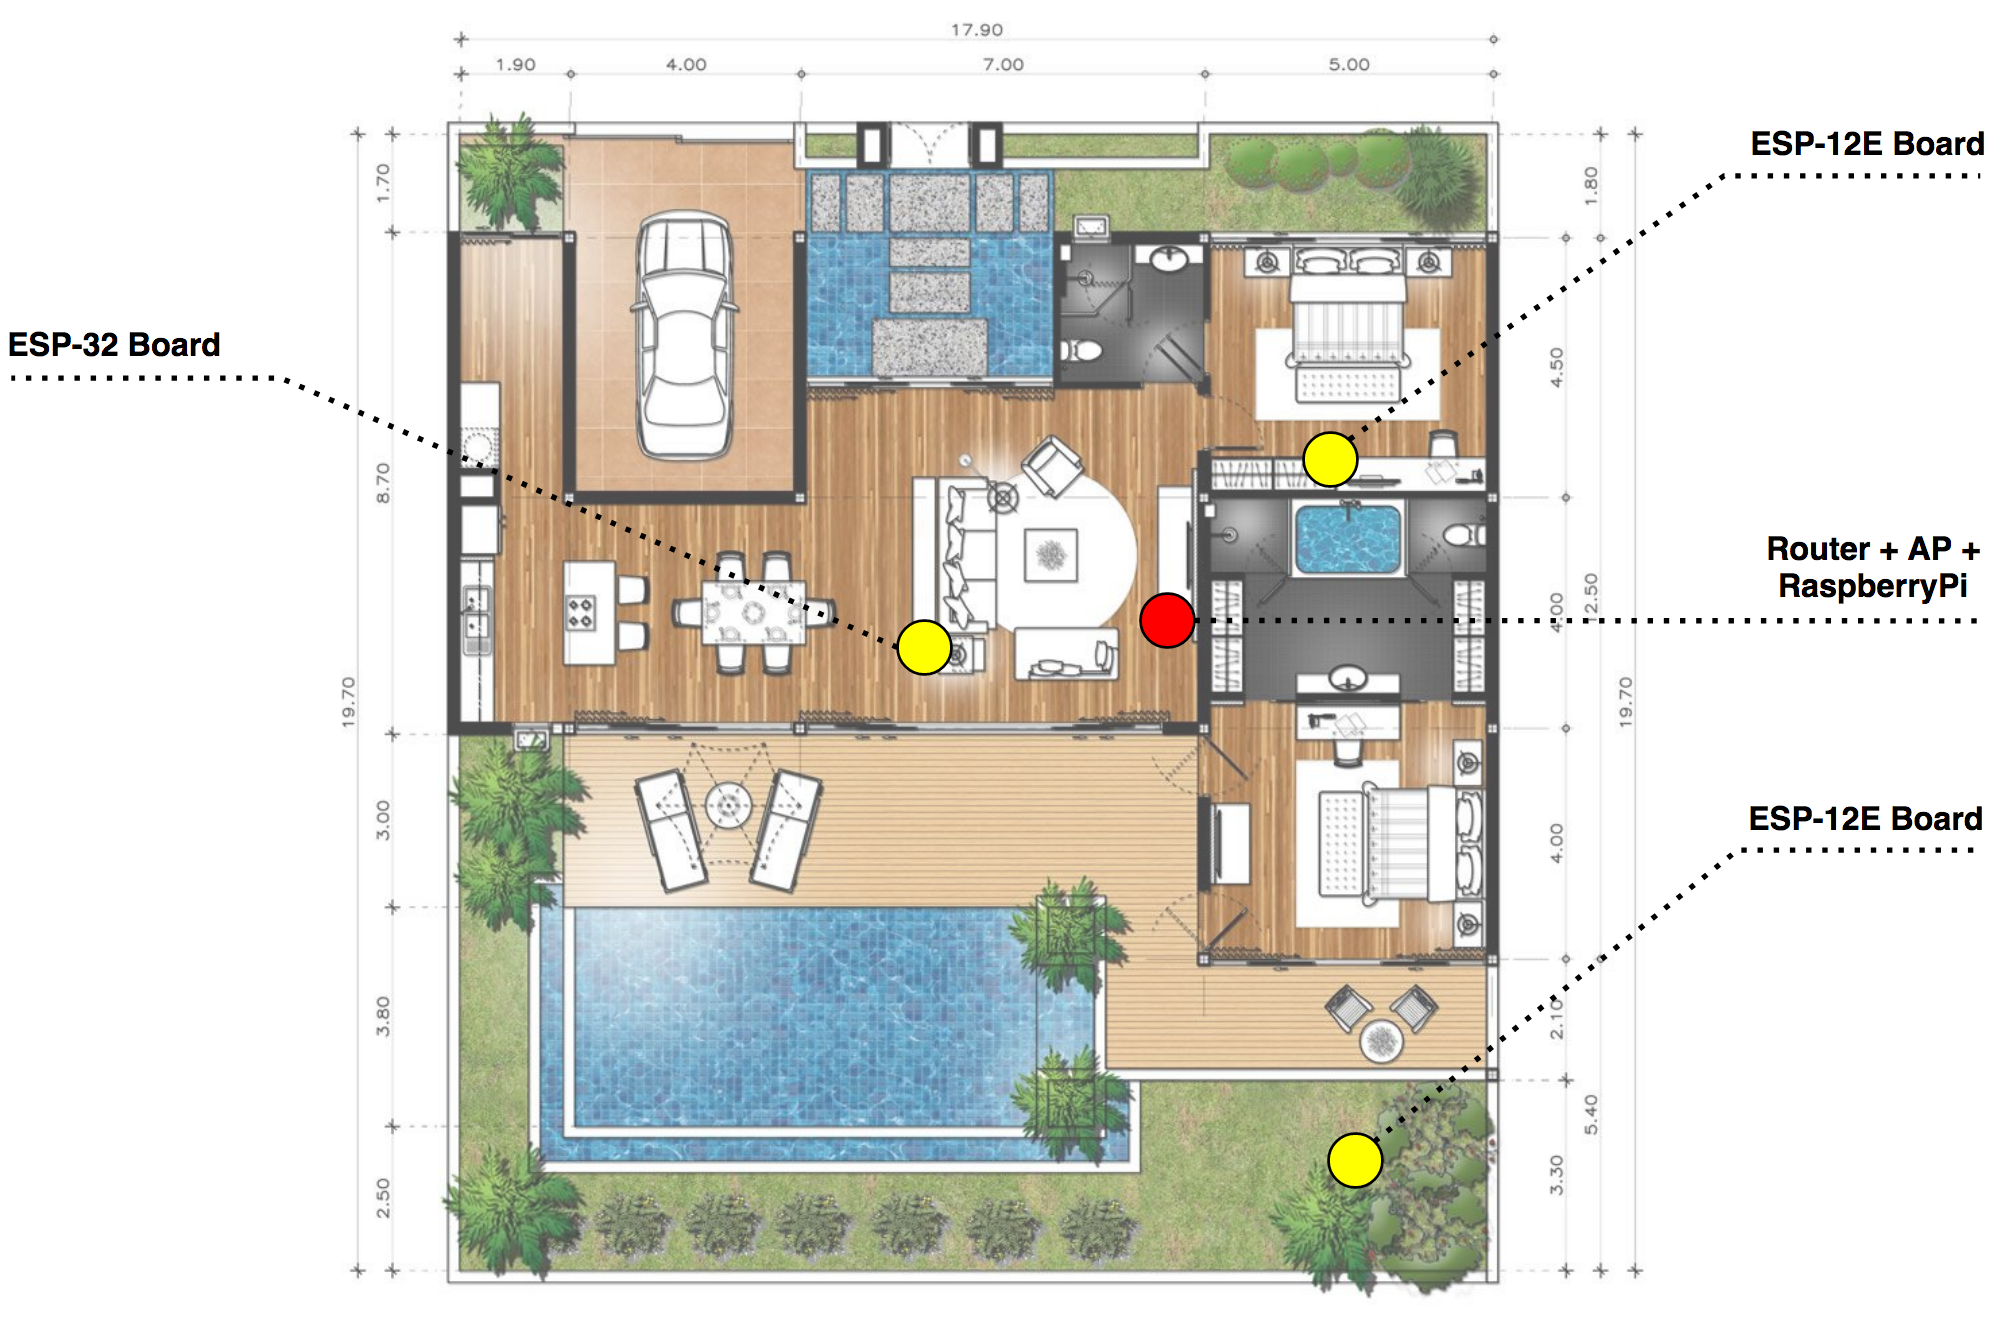
\includegraphics[width=\textwidth]{./pictures/blueprint_deployment.png}
		\caption{Blueprint of a typical house showing the position of all the system nodes.}
		\label{blueprint_deployment}
	\end{center}
\end{figure}

\section{Future Extensions}
The system implementation opens the possibility of including new features. For example:

\begin{itemize}
	\item The possibility of adding more boards to cover larger areas and collect more information about the surrounding environment;
	\item The possibility of using different sensors in addition to the simple temperature, humidity and light ones of the current implementation.
	\item The possibility of using \textit{energy harvesting} to derive energy from external sources, such as solar power and wind energy.
\end{itemize}